

\chapter{实验结果及分析}

\section{对消息的正确解析}

在 Makefile 中增加一项 test\_example 来批量测试 example,结果如图\ref{fig:maketestexample}所示。其中 Makefile 增加的脚本如下:

\begin{lstlisting}[language=C, name={Makefile: test example}]
test_example: example
@for f in $(shell ls samples); do \
	echo "=====Test file" $$f "========="; \
	./example samples/$$f | grep Segmentation --color ; \
	echo "---------------------------------------\n"; \
done
\end{lstlisting}

\subsection{结果分析}

可以看到结果只在 error2, error3, error4 和 error5 四个情况下出现了 syntax error 的返回值,因为我们在 parser.y 增加了对测试样例中的 400 做了特殊处理,所以不会出现解析错误。且在 Makefile 中将 parse.c 原本的输出给屏蔽了,所以也不会有多余输出。

\section{实现简单的 echo web server}

实验操作如下:
\begin{enumerate}
    \item 在 echo\_client 中增加直接从文件中读取的支持,以便直接使用提供的 samples;
    \item 先打开 echo\_server;
    \item 然后通过 echo\_client 发送一系列文件,查看 echo\_server 的结果。
\end{enumerate}

\subsection{实验结果截图及分析}
实验结果如图\ref{fig:echo web server}所示。可以看到,在 head, get 和 post方法的实验中,我们实现了 echo 的效果。在 400 和 501 的输入中,我们实现了相应的返回消息。在输入文件不存在时,我们也得到了相应的正确返回,体现了我们程序的鲁棒性。

\begin{figure}[htbp!]
    \centering
    \subfigure[Head get and post actions]{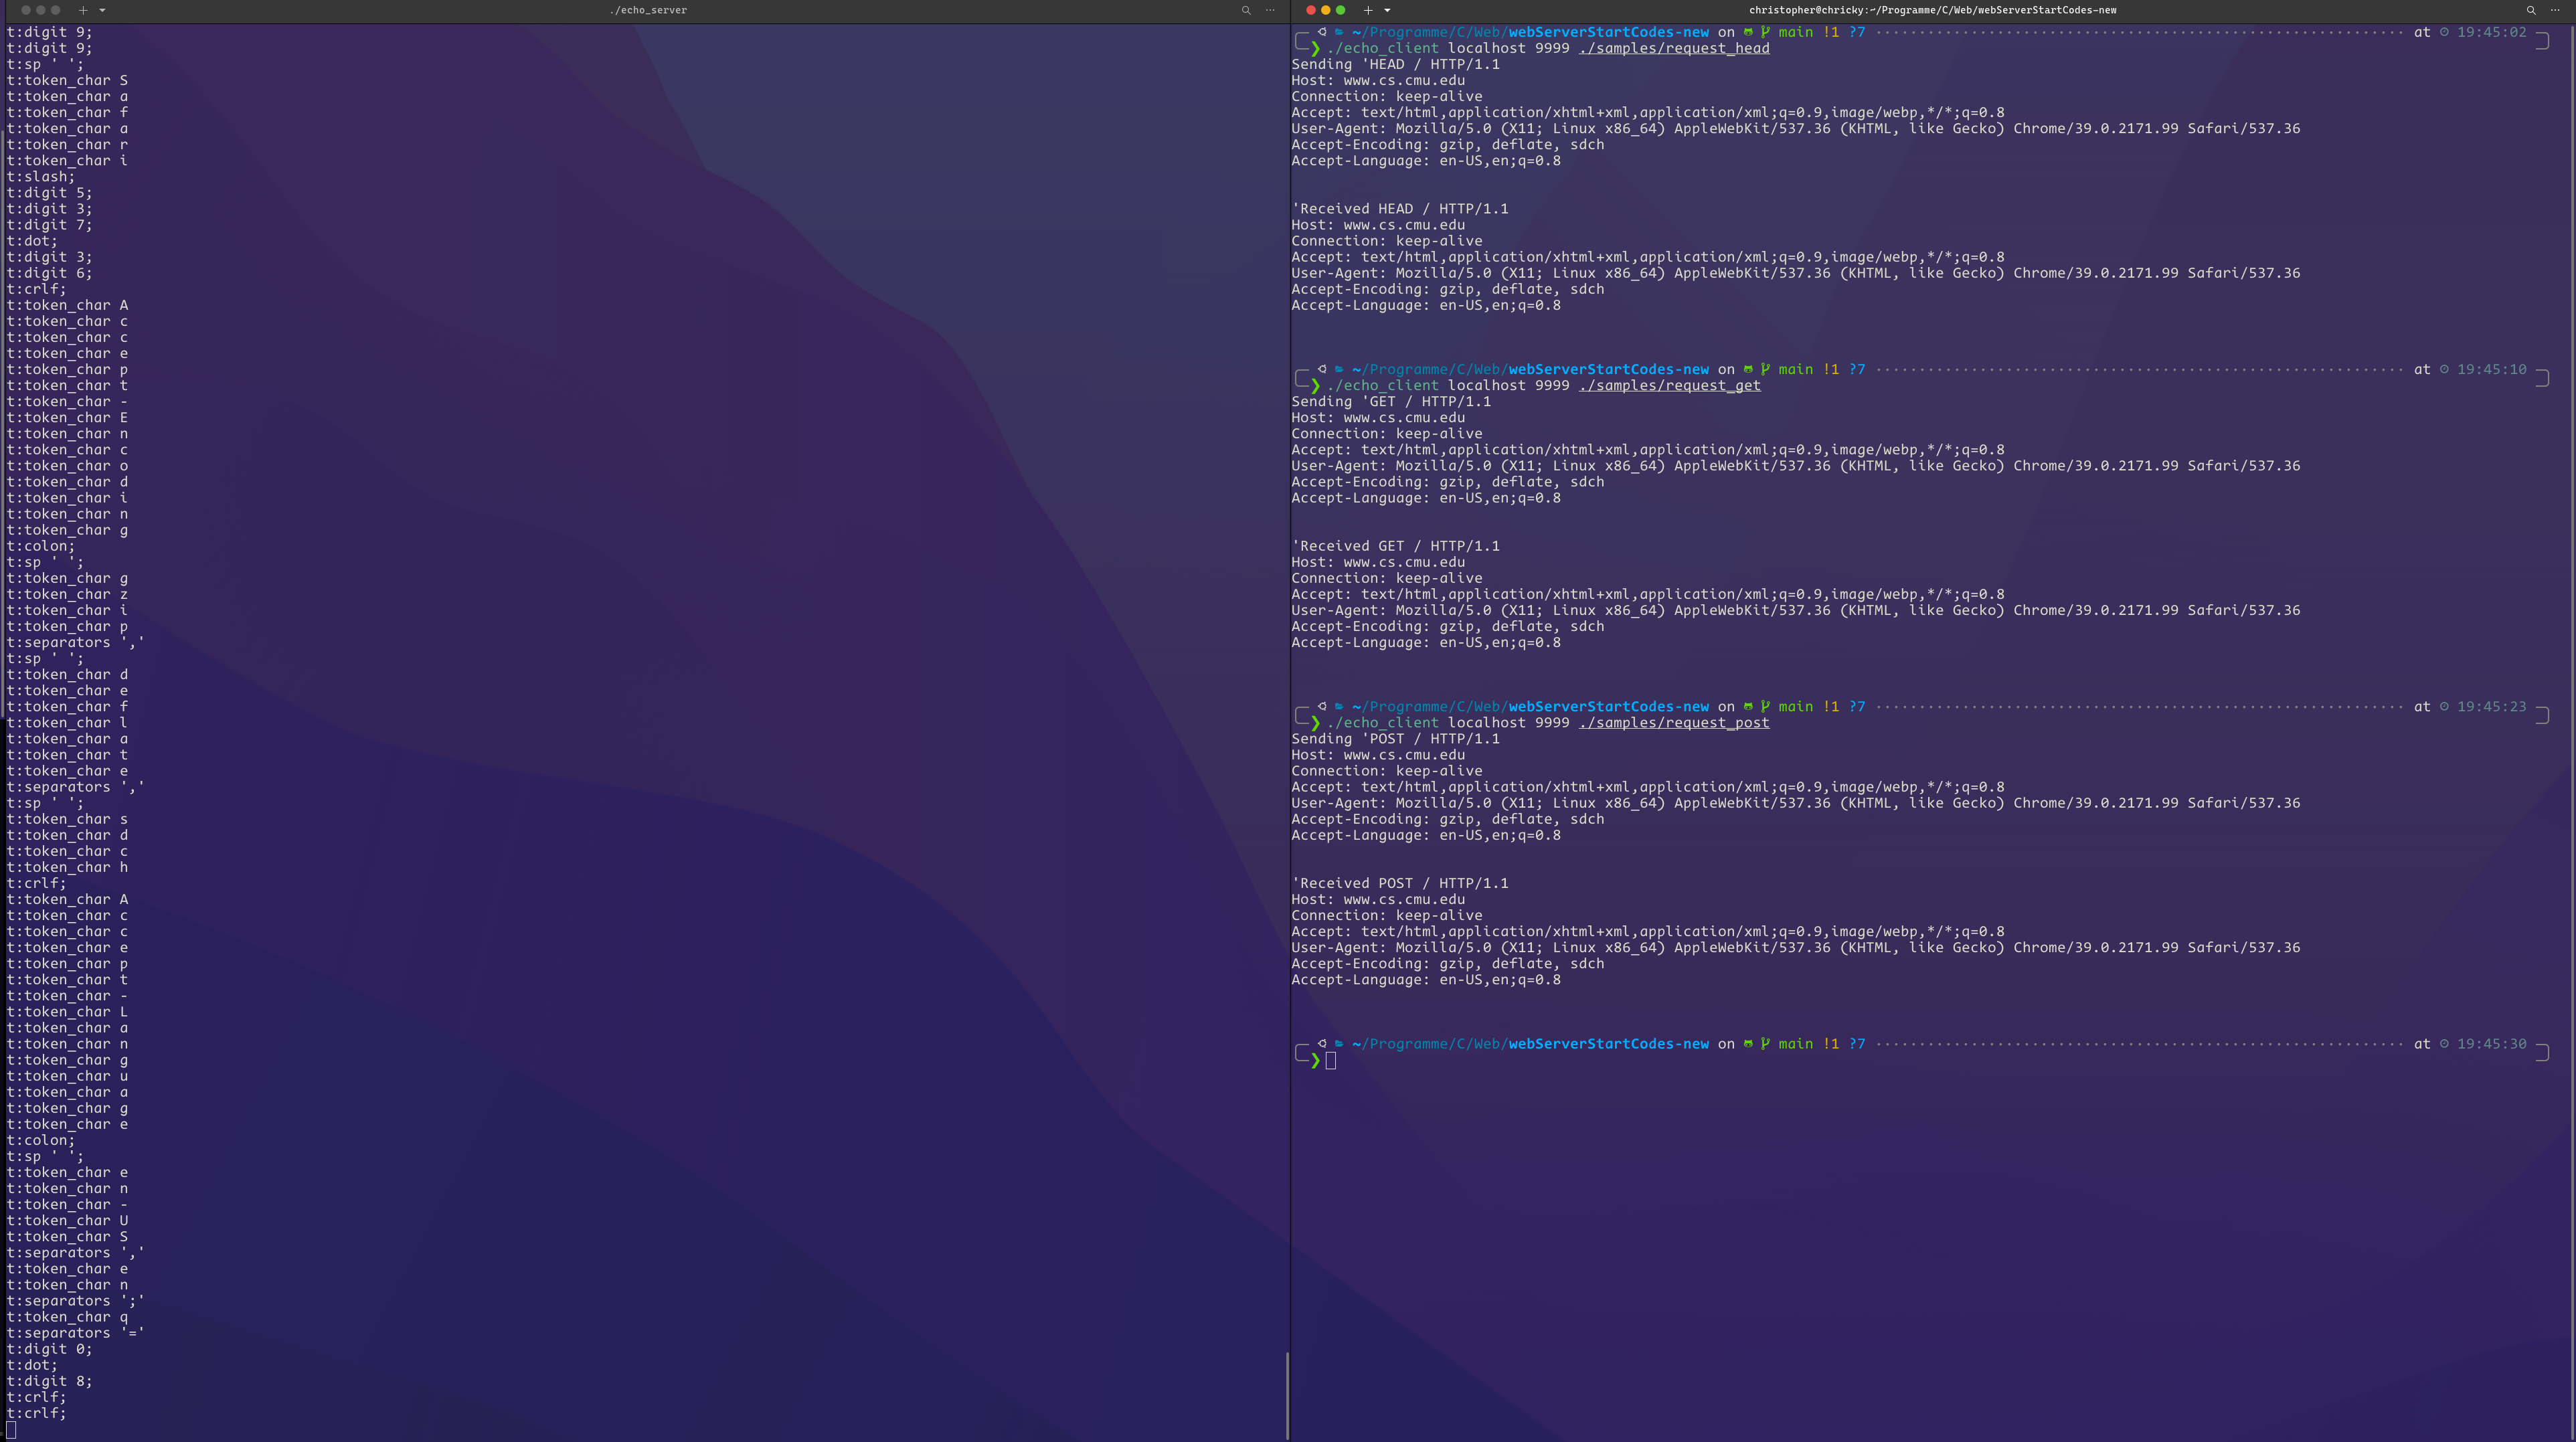
\includegraphics[width=5.7in]{head_get_post.png}}
    \subfigure[400 and 501]{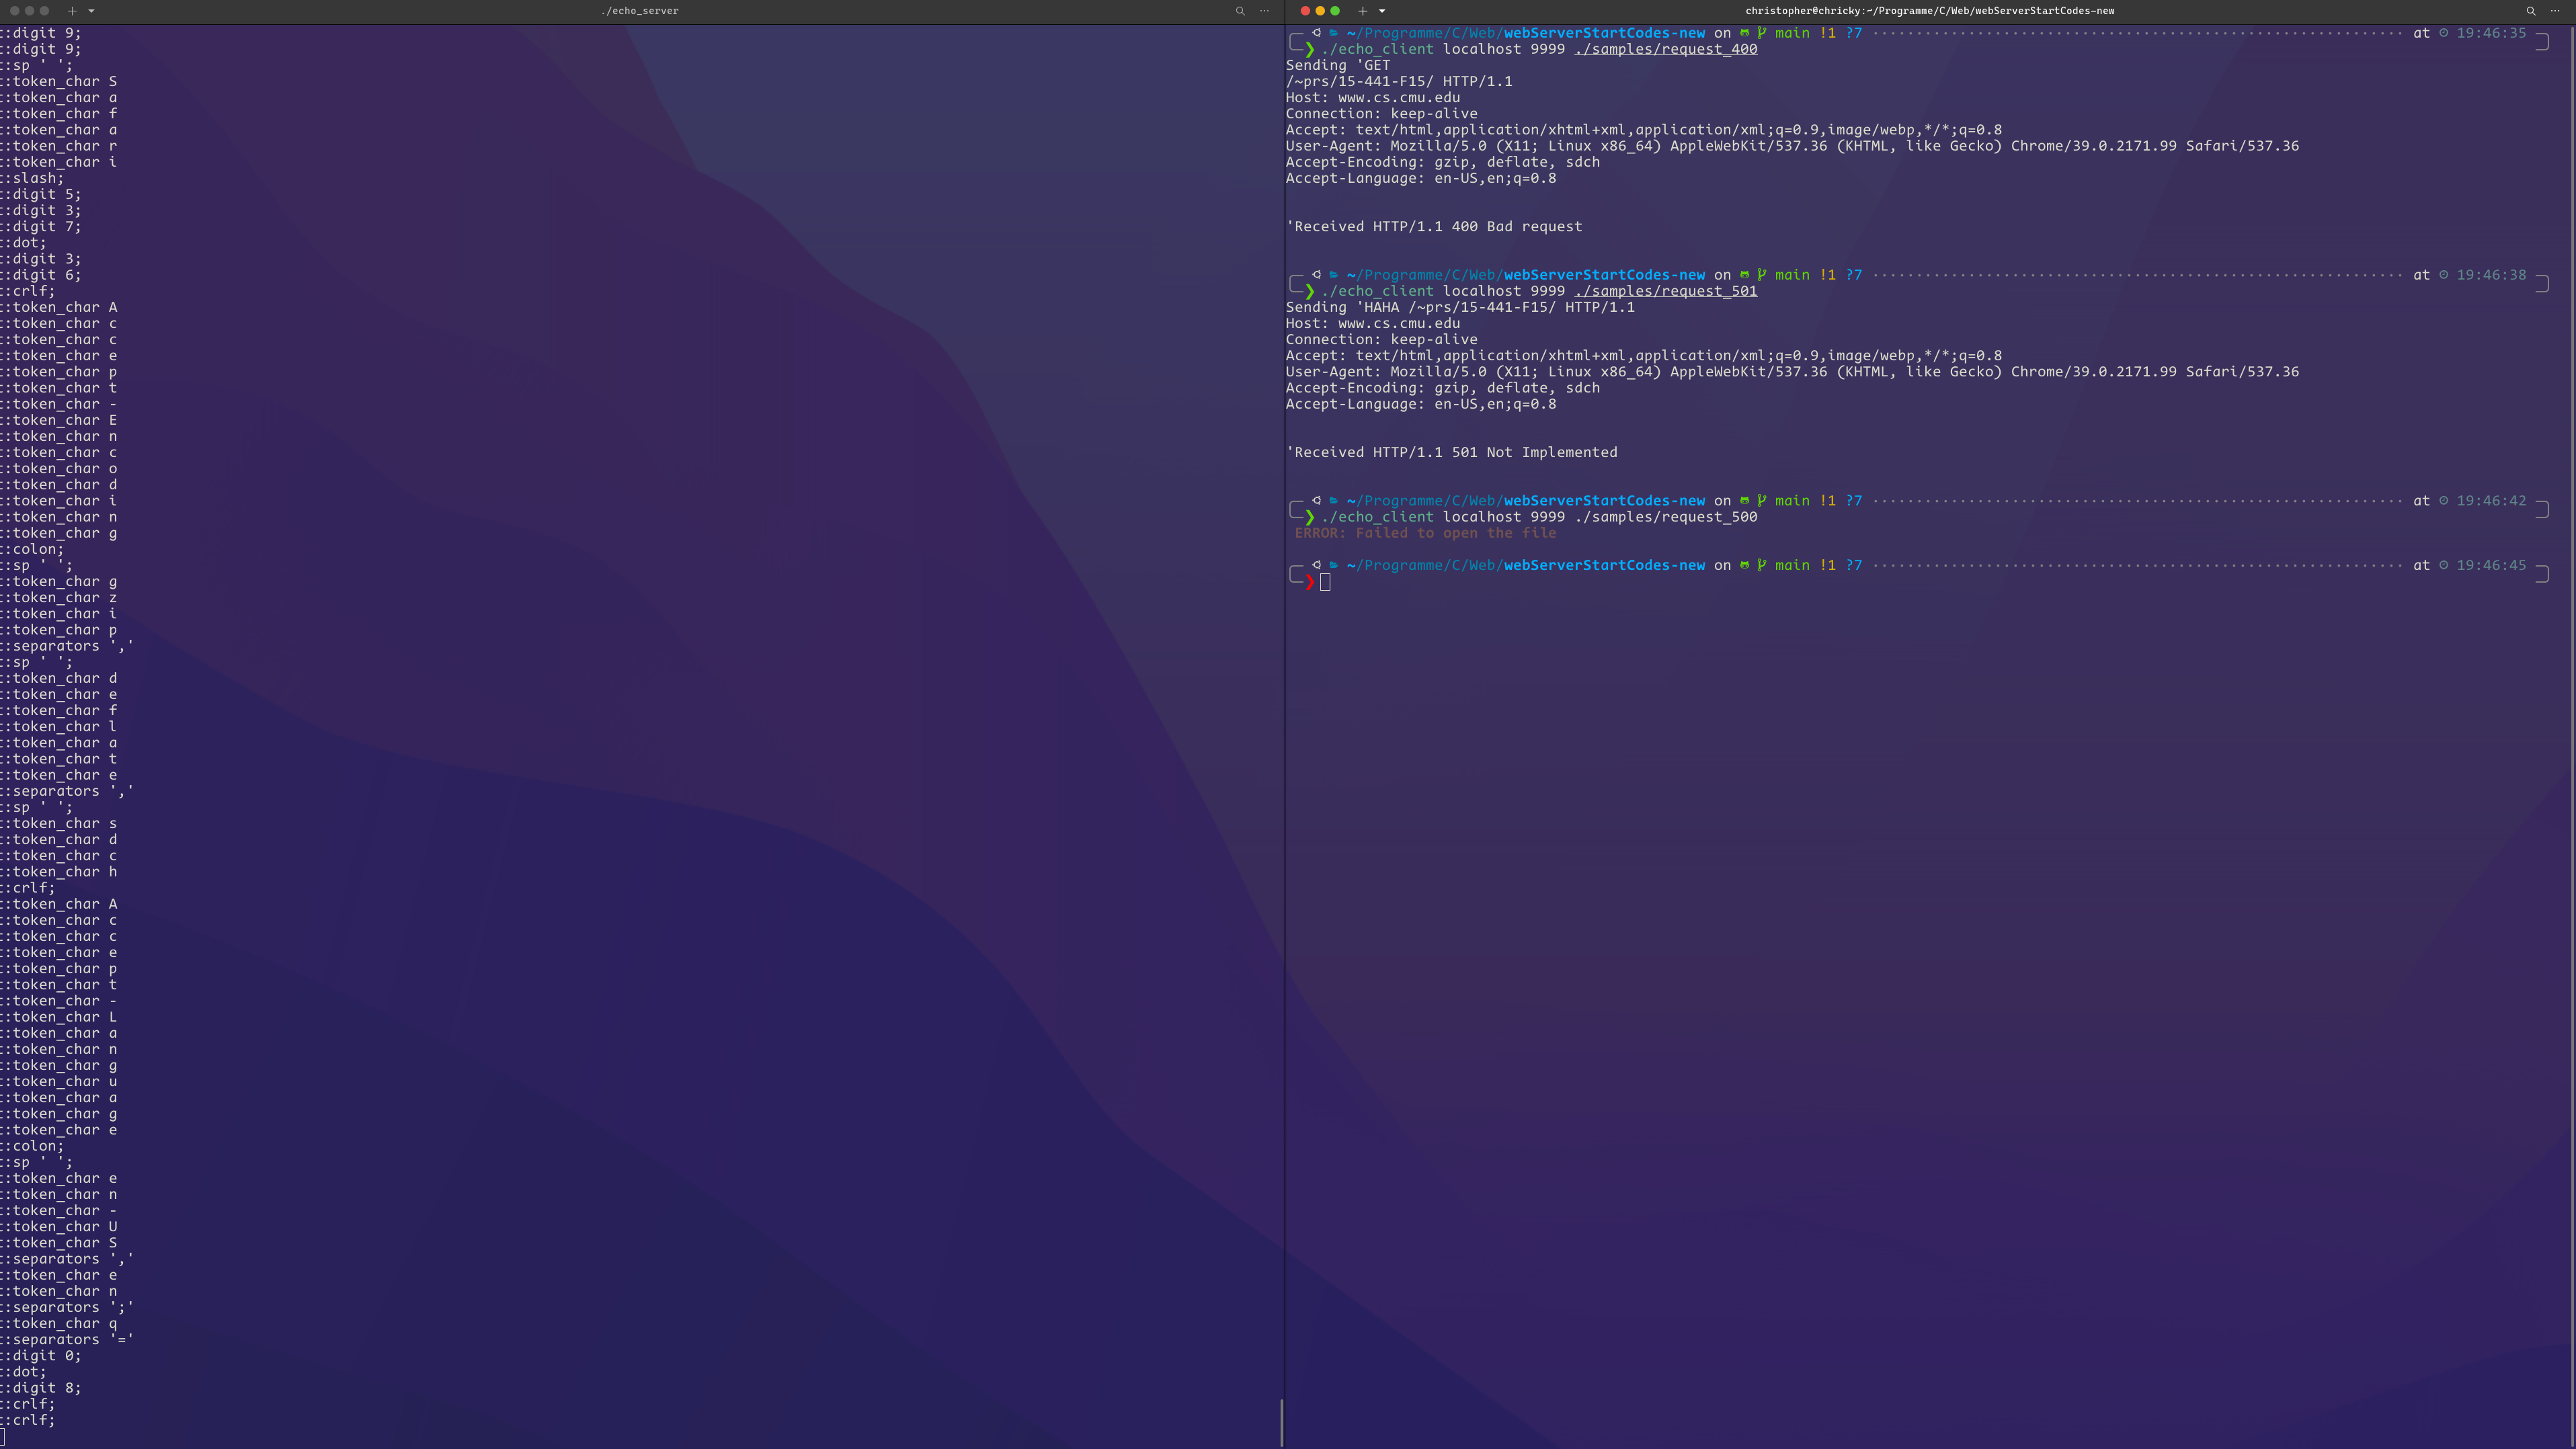
\includegraphics[width=5.7in]{400_501.png}}
    \caption{echo web server}\label{fig:echo web server}
    \vspace{-1em}
\end{figure}

\subsection{上交实验平台}
如图\ref{fig:autolab},我们的程序在第一次提交及获得了满分的成绩,且在次日稍作修改(删除部分多余代码)后依然能满分通过第一周的测试点。

\begin{figure}[htbp!]
    \centering
    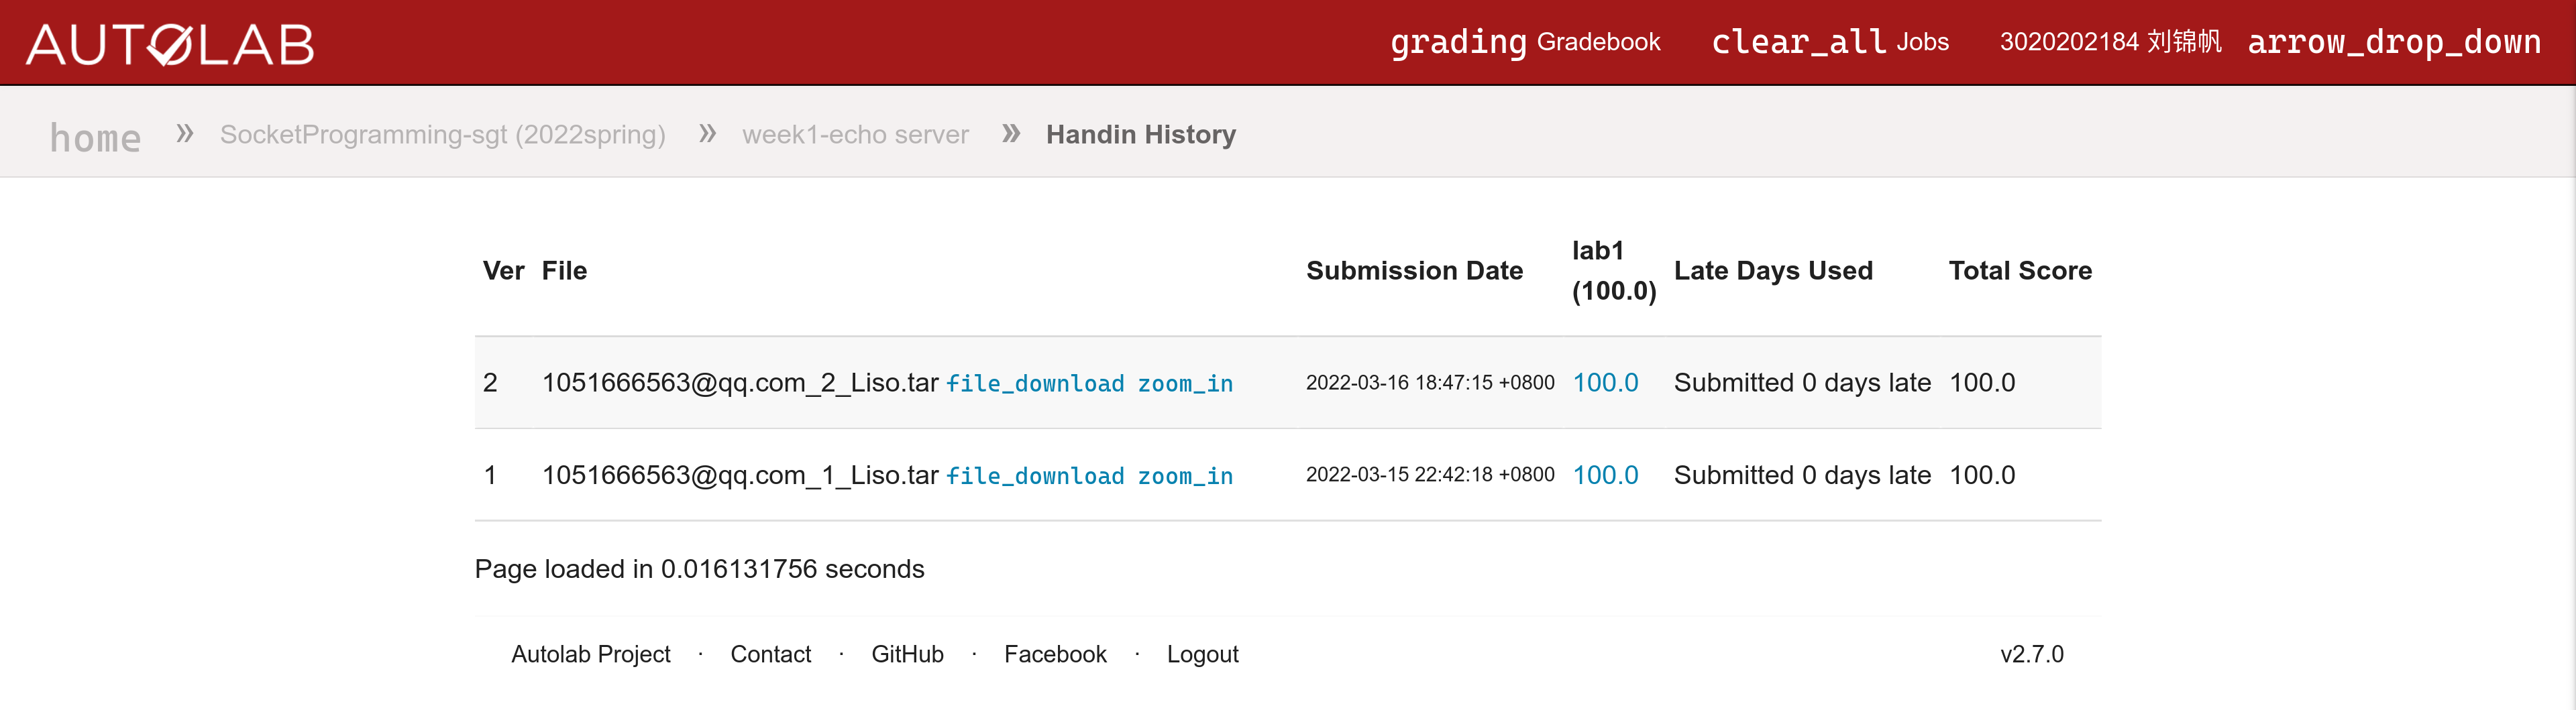
\includegraphics[width=4.5in]{autolab_uploaded.png}
    \caption{Auto Lab Confirm}\label{fig:autolab}
    \vspace{-1em}
\end{figure}
